\documentclass{strategynet-journal}

\hypersetup{
  pdftitle={Option Portfolio Selection Around Two Event Shocks},
  pdfauthor={research@strategynet.ai}
}
\newcommand{\VOLT}{\textsf{Volt}}
\newcommand{\ES}{\operatorname{ES}}

\SNHeader{strategynet.ai:Volt}
\title{Option Portfolio Selection Around Two Event Shocks\\
\large SPY Tariffs, USO Conflict Risk, and Volatility Forecasts}
\author{\href{mailto:research@strategynet.ai}{research@strategynet.ai}}
\date{July 2026}

\begin{document}
\maketitle

\begin{abstract}
This paper studies option portfolios entered before two event shocks: the April 2025 tariff escalation in SPY and the February--March 2026 US--Iran conflict in USO.  It asks two trading questions.  Given probabilities for an event and an opposing outcome, which bounded option portfolio offers the preferred directional exposure?  Given no directional view but a forecast of realized volatility, which daily delta-hedged gamma position is preferred, and are the entry options rich or cheap relative to that forecast?  Each study begins with ten liquid listed American options.  A portfolio compiler enumerates one-to-four-leg positions, applies account limits, and sends the retained candidates through pathwise American valuation, exercise, assignment, settlement, hedging, financing, and transaction costs.  Historical prices are used for the entry state and one subsequent replay; candidate selection uses only the forecasts and generated paths.  The directional tariff forecast selects concentrated downside convexity, while the conflict forecast selects a capped call spread at its stated probability.  The volatility analysis changes sign as the target moves through the entry implied-volatility level.  Deep Sets and a typed graph network are then tested as supervised surrogates for the path evaluator.  Both interpolate well within one decision date, but neither recovers a held-out optimum in the chronological development test.  Direct compiled evaluation is also faster at the portfolio counts studied here.  The empirical results support the portfolio construction and valuation procedure.  Trading-performance and learned-search claims require more independent decision dates.
\end{abstract}

\SNtwocolumntableofcontents

\section{The study}

\begin{SNcolumns}

The first decision is dated 1 April 2025.  SPY closes at \(561.03\), the
selected 11 April option expiry has a median implied volatility of \(22.20\%\),
and the tariff announcement is due the next day.  The second decision is dated
27 February 2026.  USO closes at \(81.93\), the selected 20 March expiry has a
median implied volatility of \(61.83\%\), and US--Israeli strikes begin the
following morning.

For each decision, the study produces two menus.  The directional menu
combines a baseline outcome and an event outcome at an analyst-supplied
probability.  The volatility menu fixes the median horizon return at zero,
varies annualized realized volatility, and applies a daily delta hedge.  Cash
is available in both menus with utility zero.

The recorded event path is kept out of portfolio selection.  It answers the
narrow question ``what would this marked position have done over these
dates?''  One replay cannot estimate expected return, a Sharpe ratio, or
performance across market regimes.

The analyst makes one discretionary choice at the entry close.  Later points
in the rollout are the prescribed hedge, exercise, assignment, and close
actions.  Re-selecting the portfolio through time would require a dated
series of forecast probabilities; no such series is assumed here.

\end{SNcolumns}

\section{What happened}

\subsection{Tariffs: 1--9 April 2025}

The 2 April order set a \(10\%\) additional tariff on most imports from
5 April and higher country-specific rates from 9 April.  China announced a
\(34\%\) retaliatory tariff on 4 April.  The United States raised its
additional China rate from \(34\%\) to \(84\%\) on 8 April.  On 9 April the
country-specific rates for most trading partners were paused for 90 days,
the \(10\%\) general tariff remained, and the China rate rose again to
\(125\%\) \cite{crs-tariffs}.  The S\&P 500 gained \(9.5\%\) on the pause day
but remained below its 2 April close \cite{strategynet-tariffs}.

The equity response was broad.  All eleven sector SPDRs lost value over the
2--9 April window; XLE fell \(12.5\%\), XLB \(7.2\%\), XLRE \(6.8\%\), and
XLK \(2.7\%\).  The cross-sectional mean of the 10-day price-momentum score
fell from \(-0.42\) on 3 April to \(-5.24\) on 9 April.  SPY fell from the
entry close of \(561.03\) to \(496.74\) before rebounding to \(543.37\).

\begin{figure}[H]
  \centering
  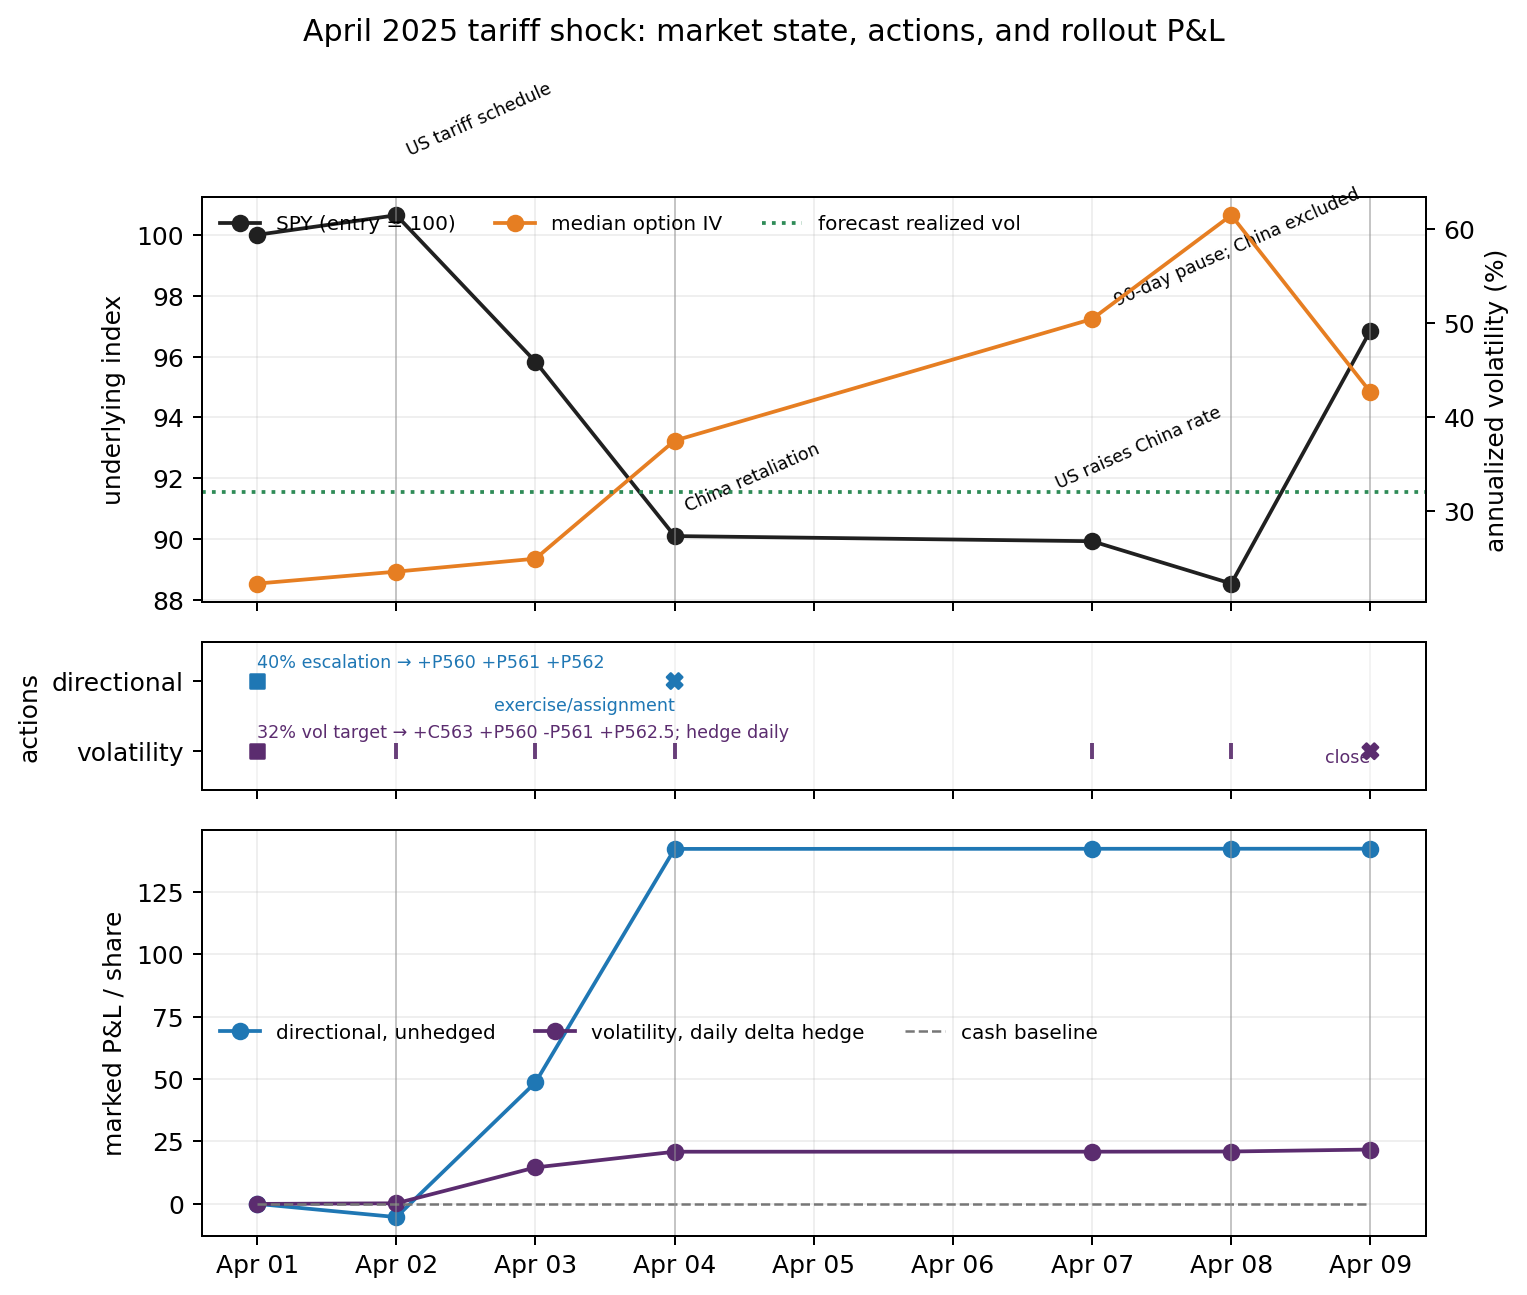
\includegraphics[width=0.94\linewidth]
    {assets/volt-event-tariff-timeline.png}
  \caption{Tariff chronology and full marked rollout.  The upper panel
  combines the indexed SPY close with median implied volatility.  The middle
  panel records entry, scheduled hedges, and exit.  The lower panel compares
  cash with the selected unhedged directional portfolio and the selected
  daily delta-hedged volatility portfolio.}
  \label{fig:tariff-timeline}
\end{figure}

The common date axis makes the market mechanics visible.  By 4 April SPY is
about ten percent below entry and median IV has risen from \(22.20\%\) to
roughly \(39\%\).  The three deep-in-the-money puts exercise at that point,
locking the directional result before the 9 April rebound.  The
delta-hedged volatility position earns about \(21\) per share during the same
spot and IV shock and then changes little.  Cash remains at zero.  A terminal
payoff chart alone would miss the exercise date, the IV expansion, and the
different management rules.

\subsection{Conflict: 27 February--13 March 2026}

Joint US--Israeli strikes began on Saturday, 28 February.  Iran responded
against Israel and US facilities across the Gulf and asserted control over
the Strait of Hormuz.  The first listed-market response came on Monday,
2 March.  Oil moved above \(100\) dollars per barrel on 9 March amid estimates
of roughly seven million barrels per day of regional production at risk
\cite{strategynet-conflict,ap-conflict}.

The market response was concentrated rather than uniform.  USO rose from
\(81.93\) on 27 February to \(119.84\) on 13 March.  The cross-sectional
dispersion of the equity volatility score rose \(27\%\) through 9 March,
while its mean declined.  The 10-day price-momentum mean initially rose from
\(0.33\) to \(0.79\), turned negative on 4 March, and reached \(-2.13\) by
13 March.  Those factor statistics describe the broader equity distribution;
the option decision below concerns USO.

These dates organize descriptive market replays.  Estimating the causal
effect of either event would require controls for concurrent news and market
conditions.

\begin{figure}[H]
  \centering
  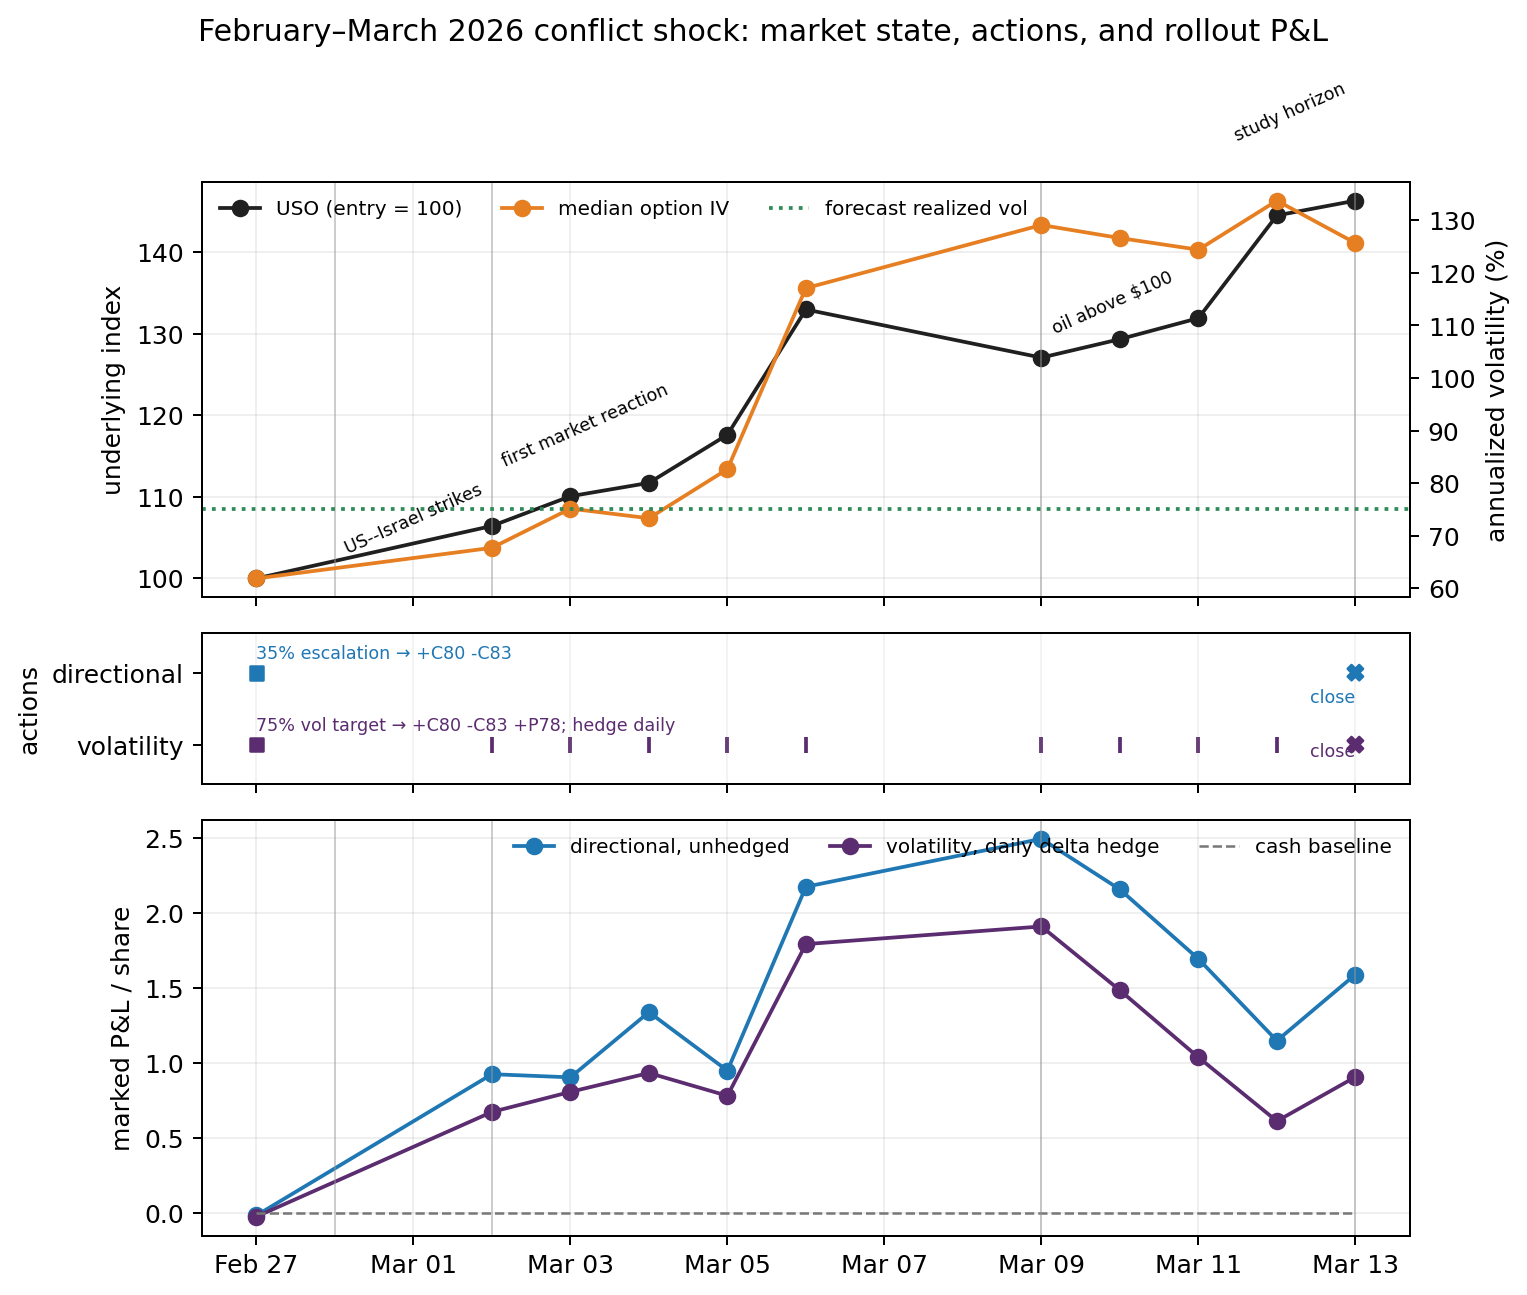
\includegraphics[width=0.94\linewidth]
    {assets/volt-event-conflict-timeline.png}
  \caption{Conflict chronology and full marked rollout.  Market state,
  portfolio actions, cash, the selected directional position, and the
  selected volatility position share one date axis.}
  \label{fig:conflict-timeline}
\end{figure}

Figure~\ref{fig:conflict-timeline} shows why a correct directional call can
still have a non-monotone marked result.  The \(80/83\) call spread reaches
about \(2.49\) per share on 9 March, then falls to \(1.59\) even as USO rises
further.  Once both calls are deep in the money, the spread converges toward
its three-point cap while time and the relative marks of its two legs change.
The delta-hedged volatility position follows the same early shock, peaks near
\(1.91\), and closes at \(0.91\).  The common timeline separates a correct
market direction from the path of a particular option structure.

\section{Market data and option valuation}

The underlying close and option state are synchronized at 16:00 New York.
The chain filter selects five calls and five puts from one expiry using only
entry-date moneyness, volume, and transaction count.  Every contract in the
study is a physically settled American option with multiplier \(100\).

Some option series do not print at exactly 16:00.  For each contract and day,
the loader takes the implied volatility from the last valid regular-session
minute and revalues the contract at the synchronized underlying close.
A same-right strike interpolation supplies the volatility when the selected
contract has no valid minute observation.  The recorded option marks and
their source files are fingerprinted.

American contracts are valued with a Cox--Ross--Rubinstein lattice
\cite{crr}.  At every path observation the evaluator checks the exercise
value against continuation value.  Long exercise and short assignment alter
cash and underlying inventory; physical settlement and the fixed-horizon
close are then applied.  A European contract is the special case whose
exercise set contains only expiry.  The present empirical chains contain
American contracts throughout.

The option-cost assumption is \(0.65\) dollars per contract side.  The
delta-hedged study also charges one basis point for underlying trades.
Results are reported in option-price units per share; multiplying by the
contract multiplier converts one unit of quantity to dollars.  The marks do
not reconstruct a fill at the bid or offer, so the reported replay is a
marked implementation study rather than an executable fill record.

\begin{table}[H]
\centering
\small
\begin{tabular}{@{}p{0.20\linewidth}p{0.35\linewidth}p{0.35\linewidth}@{}}
\toprule
 & Tariff study & Conflict study \\
\midrule
Underlying & SPY & USO \\
Entry close & 1 April 2025 & 27 February 2026 \\
Evaluation horizon & 9 April 2025 & 13 March 2026 \\
Option expiry & 11 April 2025 & 20 March 2026 \\
Entry spot & \(561.03\) & \(81.93\) \\
Median entry IV & \(22.20\%\) & \(61.83\%\) \\
Contracts & five calls, five puts & five calls, five puts \\
Raw candidates & \(2{,}890\) & \(2{,}890\) \\
Directional candidates & \(1{,}675\) & \(598\) \\
Volatility candidates & \(789\) & \(414\) \\
\bottomrule
\end{tabular}
\caption{Point-in-time decision states.  Different retained counts reflect
the same account limits applied to different marks and payoff geometry.}
\label{tab:decision-states}
\end{table}

\section{Portfolio construction and objectives}

\subsection{From contracts to candidates}

Let \(q_j\in\{-1,0,+1\}\) be the quantity of contract \(j\).  A candidate is
the nonzero vector \(q=(q_1,\ldots,q_J)\) with at most four active entries.
Canonicalization means that quantities are keyed by contract identifier,
duplicate references to one contract are netted, zero positions are removed,
and the remaining legs are sorted.  Two input lists that differ only in leg
order therefore produce one candidate.

The compiler rejects unbounded expiration loss and expiration loss above
five percent of entry spot.  The volatility menu adds
\[
  |\Delta_0(q)|\leq 0.20,\qquad
  |\Gamma_0(q)|\geq 10^{-5},\qquad
  |\mathcal V_0(q)|\geq 10^{-4},
\]
where vega is measured per one-point change in absolute volatility.  Delta,
gamma, theta per calendar day, and vega are signed sums of the contract
sensitivities.  Strategy names are descriptive labels applied after
selection; they do not restrict the search.  Expiration diagrams use the
standard long/short call and put payoff conventions \cite{occ}.

\subsection{Directional forecast}

The two directional outcomes in Table~\ref{tab:forecast-inputs} specify a
median horizon return, annualized spot volatility, and terminal multiplier
for the entry implied-volatility surface.  Each outcome contributes 256
paths.  Spot follows geometric Brownian motion at the observed dates.  A
common, mean-reverting implied-volatility factor has annual volatility
\(1.0\), mean reversion \(8.0\), and correlation \(-0.60\) with the spot
shock.  The portfolio is held without a delta hedge, subject to the
American lifecycle rules.

\begin{table}[H]
\centering
\small
\begin{tabular}{@{}p{0.19\linewidth}p{0.36\linewidth}p{0.36\linewidth}@{}}
\toprule
 & Baseline outcome & Event outcome \\
\midrule
Tariff &
\(60\%\) probability; \(+1\%\) median SPY return; \(16\%\) volatility;
terminal IV multiplier \(0.90\) &
\(40\%\) probability; \(-7\%\) median SPY return; \(32\%\) volatility;
terminal IV multiplier \(1.30\) \\
Conflict &
\(65\%\) probability; \(-5\%\) median USO return; \(45\%\) volatility;
terminal IV multiplier \(0.85\) &
\(35\%\) probability; \(+20\%\) median USO return; \(75\%\) volatility;
terminal IV multiplier \(1.25\) \\
\bottomrule
\end{tabular}
\caption{Declared forecast inputs.  They are decision assumptions, not
parameters estimated from the subsequent event path.}
\label{tab:forecast-inputs}
\end{table}

For candidate \(q\), pathwise net P\&L at the fixed horizon is
\(P(q,\omega)\).  The ranking statistic under the stated outcome
probabilities is
\[
  U(q)=\mathbb E[P(q,\omega)]
       +0.25\,\ES_{0.10}[P(q,\omega)],
\]
where \(\ES_{0.10}\) is the signed mean of the lowest ten percent of P\&L.
Cash has \(U=0\).  The \(0.25\) coefficient is a declared risk preference.

\subsection{Direction-neutral volatility forecast}

The volatility menu uses the same entry chain and candidate compiler, sets
the median horizon return to zero, and holds each contract's entry implied
volatility constant along a path.  Annualized realized volatility is scanned
from \(0.45\) to \(1.60\) times the median entry IV, with the event-study
target inserted into the grid.  Each target has 64 generated paths.  The
option position is delta-hedged at every daily observation.  The target
levels share the same standardized spot shocks, so movement across the scan
comes from the volatility assumption rather than a new Monte Carlo sample.

This setup gives ``rich'' and ``cheap'' precise meanings.  A target below the
entry IV treats the options as rich relative to the forecast; a target above
entry IV treats them as cheap.  The conclusion is conditional on the chosen
target, constant-IV marking rule, hedge frequency, transaction costs, and
candidate limits.  Gamma P\&L, theta P\&L, vega P\&L, the delta hedge,
financing, costs, and the lattice residual reconcile to net P\&L on every
path.  ``Rich'' and ``cheap'' are shorthand for the target's relation to
median IV; every leg is still valued from its own entry IV and strike.

\section{Surrogate models}

\begin{SNcolumns}

The path evaluator supplies four labels for each portfolio:
\[
  y(q)=\left(
    \mathbb E[P],\
    \ES_{0.10}[P],\
    \operatorname{sd}(P),\
    \Pr(P>0)
  \right).
\]
The learned models estimate these labels.  Utility is calculated from the
first two predicted components; it is not a separate training target.

For Deep Sets \cite{deepsets}, each active option leg has a 14-element feature
vector containing signed quantity, call/put, log moneyness, mark divided by
spot, implied volatility, liquidity, multiplier, exercise and settlement
flags, and the leg's signed entry Greeks.  Shared context contains time to
expiry, rate, dividend yield, and the forecast fields.  The network is
\[
  \widehat y(q,c)
  =\rho\!\left(\sum_{j:q_j\ne0}\phi(x_j),c\right),
\]
where \(\phi\) and \(\rho\) are two-layer SiLU multilayer perceptrons with
48 hidden units.  The sum makes the prediction invariant to leg order.

The relation graph contains a portfolio node, an underlying node, an expiry
node, and one option-position node per active leg.  Directed typed edges
represent \emph{position in portfolio}, \emph{written on underlying}, and
\emph{expires at}, together with their reverse directions.  Position nodes
carry the same market and Greek information as the set model, while
portfolio, underlying, and expiry data reside on their own nodes.  Two
message-passing layers use relation-specific weights
\cite{graphnetworks}:
\[
  \begin{aligned}
  m_v^{(k)}
    &=\sum_{(u,v,r)\in E}W_r^{(k)}h_u^{(k)},\\
  h_v^{(k+1)}
    &=\operatorname{LN}\!\left(
       h_v^{(k)}
       +\operatorname{SiLU}(W_0^{(k)}h_v^{(k)}+m_v^{(k)})
     \right).
  \end{aligned}
\]
The four outputs are read from the final portfolio-node state and the shared
context.  Hidden width is 20.  This graph can later represent multiple
underlyings, expiries, inventory, exercise opportunities, and account
relations without flattening them into one leg set.  In the present
single-underlying, single-expiry portfolios, Deep Sets already matches the
mathematical symmetry of the problem.

The candidate-holdout experiment initially evaluates \(20\%\) of the
portfolios, uses part of that set for early stopping, and asks the model to
select another \(10\%\) for path evaluation.  Smooth-L1 loss fits standardized
labels with AdamW.  A ridge regression over summed leg features supplies a
linear baseline.  The chronological experiment trains on one earlier
decision date, selects the checkpoint on a middle date, and evaluates the
final date once.

The compiler, path engine, and learned ranking have separate jobs:
\[
\begin{aligned}
\text{contracts and limits}
  &\longrightarrow \text{candidate portfolios}\\
  &\longrightarrow \text{pathwise labels}\\
  &\longrightarrow \text{learned shortlist}.
\end{aligned}
\]
There is no reinforcement-learning result in this paper.  The models here are
supervised regressors over a fixed action set.

\end{SNcolumns}

\section{Tariff results}

\subsection{Directional view}

At \(40\%\) escalation probability, exhaustive evaluation and all three
surrogates select
\[
  +P(560)+P(561)+P(562).
\]
The entry debit and expiration maximum loss are \(24.1600\) per share.
Entry delta is \(-1.4571\), gamma \(0.0660\), daily theta \(-1.2099\), and
vega \(1.1069\) per volatility point.  Scenario-mixture utility is
\(14.3761\).

\begin{figure}[H]
  \centering
  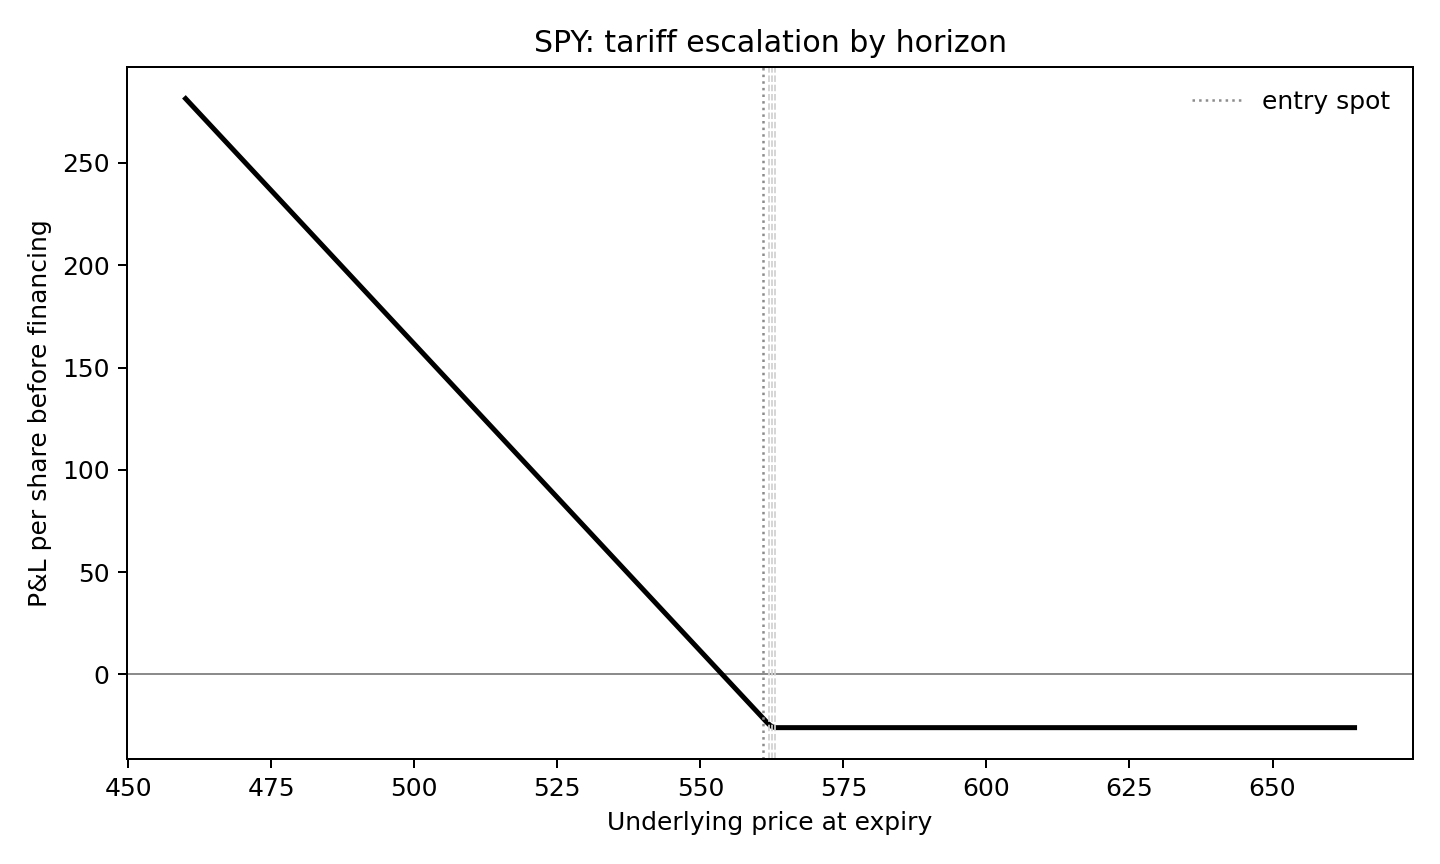
\includegraphics[width=0.86\linewidth]
    {assets/volt-event-tariff-payoff.png}
  \caption{Expiration P\&L of the tariff-escalation portfolio.  Three
  adjacent long puts concentrate downside convexity and cap loss at the
  premium paid.}
  \label{fig:tariff-payoff}
\end{figure}

Under the pure escalation outcome, the preferred strikes move to \(562\),
\(562.5\), and \(563\).  Conditional mean P\&L is \(69.4431\), the
lowest-decile mean is \(-15.9433\), and utility is \(65.4573\).  Under the
baseline outcome the same position has mean P\&L of \(-12.2214\).  It first
beats cash on the one-percentage-point probability grid at \(23\%\)
escalation probability.

\begin{figure}[H]
  \centering
  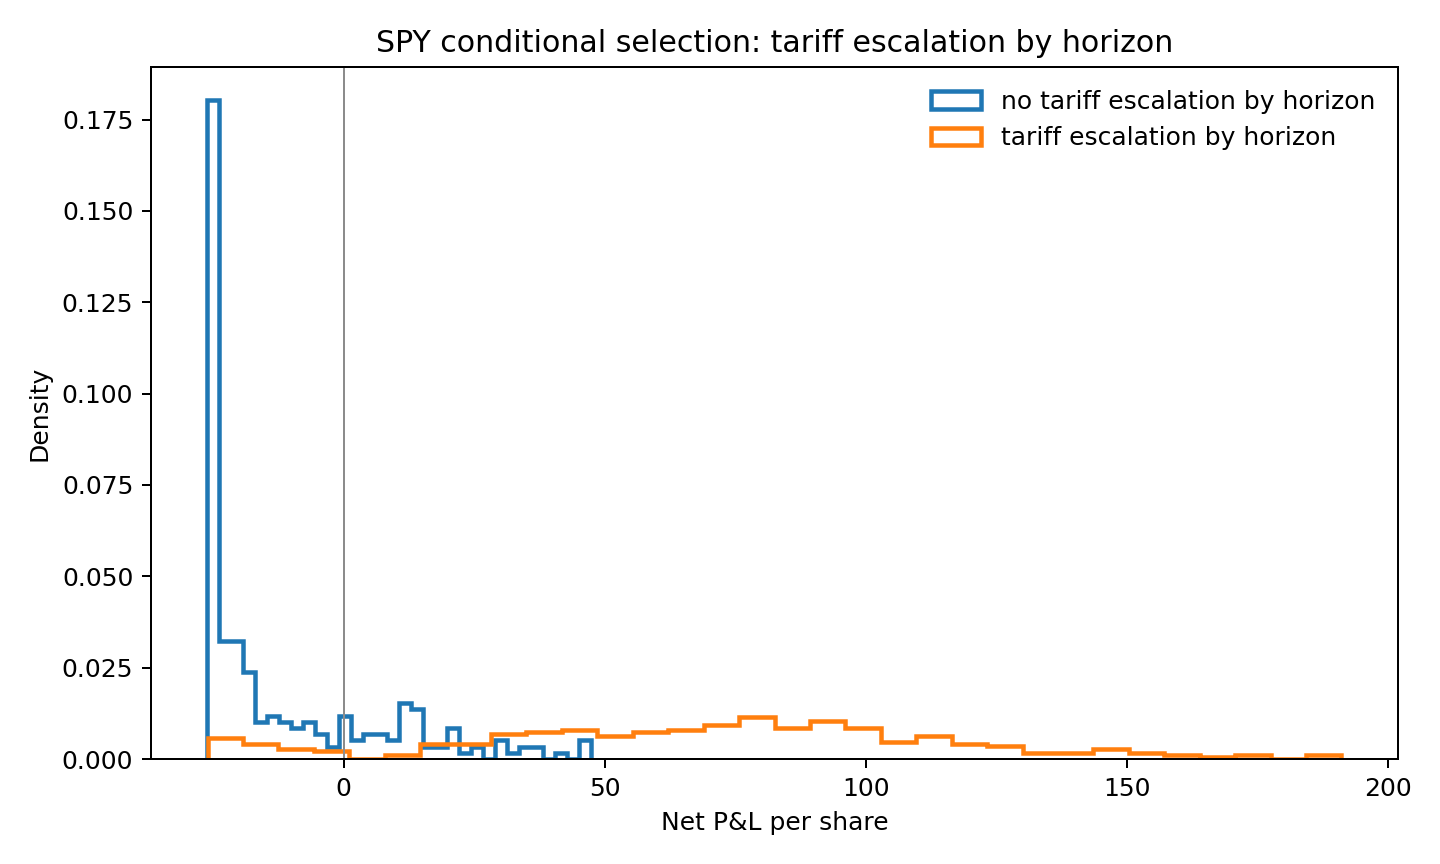
\includegraphics[width=0.87\linewidth]
    {assets/volt-event-tariff-pnl.png}
  \caption{Fixed-horizon P\&L of the pure-escalation tariff portfolio under
  the opposing forecast outcomes.}
  \label{fig:tariff-pnl}
\end{figure}

The \(40\%\)-mixture position earns \(142.3710\) per share on the recorded
path.  All three puts exercise during the selloff, so the lifecycle ledger
does not treat them as live options only at the 9 April rebound.  The
pure-escalation portfolio earns \(145.0551\) and is also the hindsight
leader.  Forecast utility and recorded-path P\&L have Spearman correlation
\(0.9478\) across the retained portfolios.

\begin{figure}[H]
  \centering
  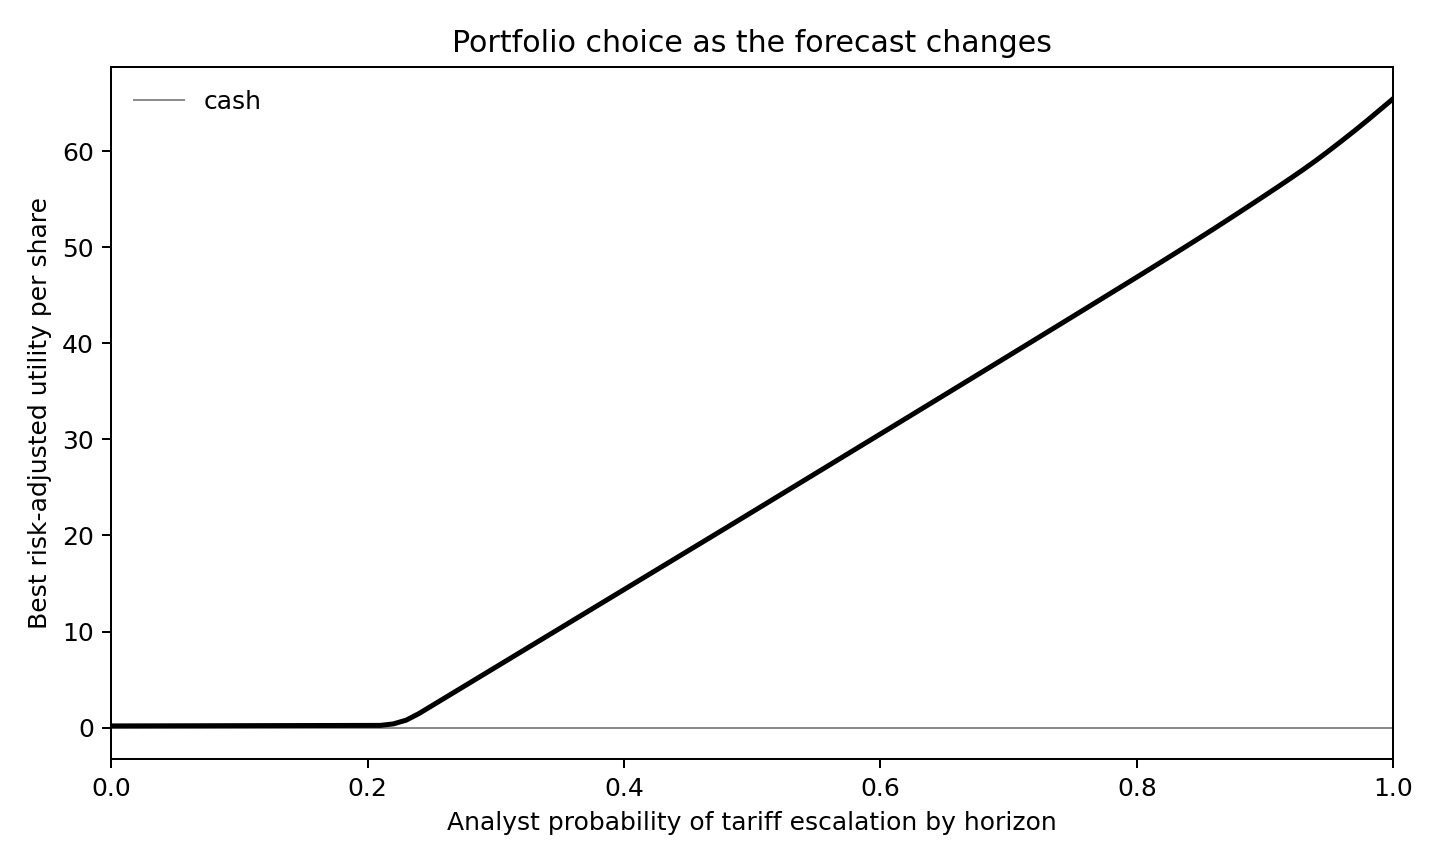
\includegraphics[width=0.88\linewidth]
    {assets/volt-event-tariff-probability.png}
  \caption{Best directional utility as tariff-escalation probability changes.
  Breakpoints mark changes in the preferred listed portfolio.}
  \label{fig:tariff-probability}
\end{figure}

\subsection{Volatility without a directional view}

At entry, the median IV is \(22.20\%\).  Close-to-close realized volatility
over the subsequent observations is \(88.70\%\).  The explicit
\(32\%\) target from the tariff event state is above the entry IV, so this
forecast treats convexity as cheap.  The preferred delta-hedged position is
\[
  +C(563)+P(560)-P(561)+P(562.5).
\]
Its entry delta is \(-0.0256\), gamma is \(0.01929\), daily theta is
\(-0.8242\), and vega is \(0.7371\).  Forecast utility is \(2.5318\), and
recorded net P\&L is \(21.7708\) per share.  On the recorded path, gamma
contributes \(34.4177\), vega \(6.0007\), theta \(-2.6304\), and the delta
hedge \(-19.8633\), before the remaining financing, residual, and cost
components.

The unrestricted optimum is short gamma through the \(25.53\%\) grid point
and long gamma from \(28.87\%\) upward.  The switch occurs above median entry
IV because skew, bounded-loss geometry, costs, the lower-tail penalty, and
daily hedge error enter alongside the scalar volatility comparison.

\begin{figure}[H]
  \centering
  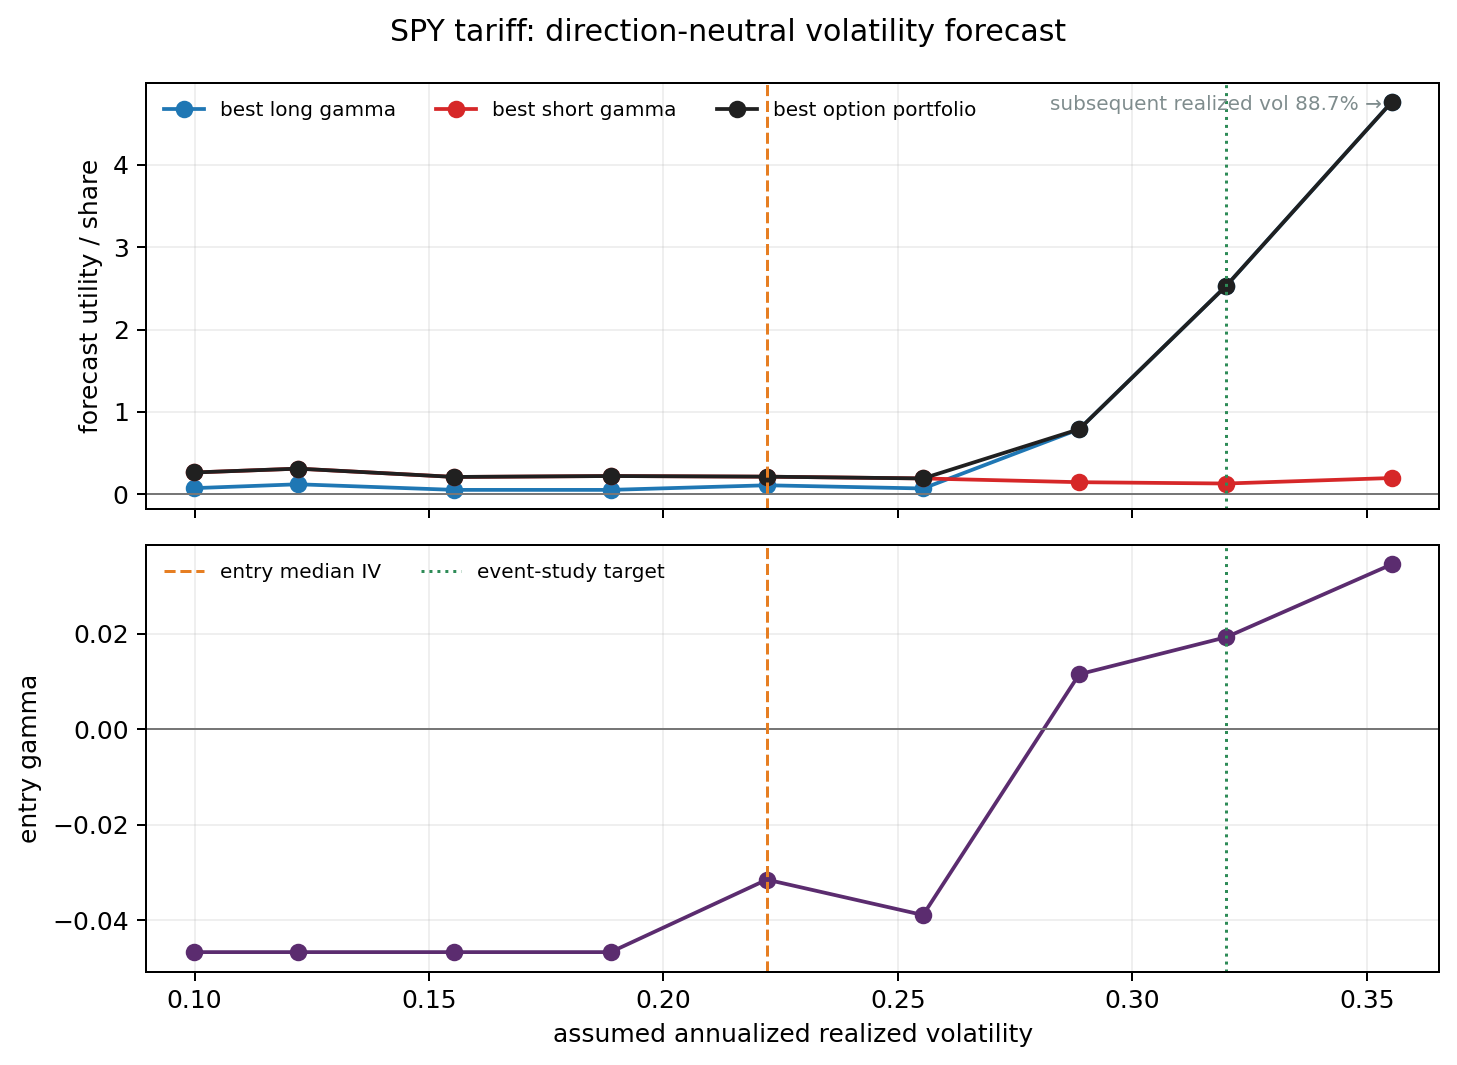
\includegraphics[width=0.90\linewidth]
    {assets/volt-event-tariff-volatility-scan.png}
  \caption{SPY target-volatility scan.  The upper panel compares the best
  long-gamma, short-gamma, and unrestricted option candidates with cash.
  The lower panel shows the entry gamma of the selected candidate.}
  \label{fig:tariff-volatility}
\end{figure}

\section{Conflict results}

\subsection{Directional view}

At \(35\%\) escalation probability, the preferred portfolio is
\[
  +C(80)-C(83).
\]
The debit and expiration maximum loss are \(1.0600\) per share; maximum
expiration profit is \(1.9400\).  Forecast utility is \(0.1318\), and the
recorded-path P\&L is \(1.5902\).

The pure escalation outcome selects
\[
  +C(80)-C(83)+P(76)-P(80).
\]
The call vertical supplies capped upside.  The short \(80\) put and long
\(76\) put contribute premium and bounded downside.  Entry delta is
\(0.2274\), gamma \(0.000073\), daily theta \(0.0332\), and vega
\(-0.0126\) per point.  This is primarily a directional structure rather
than a long-volatility position.

\begin{figure}[H]
  \centering
  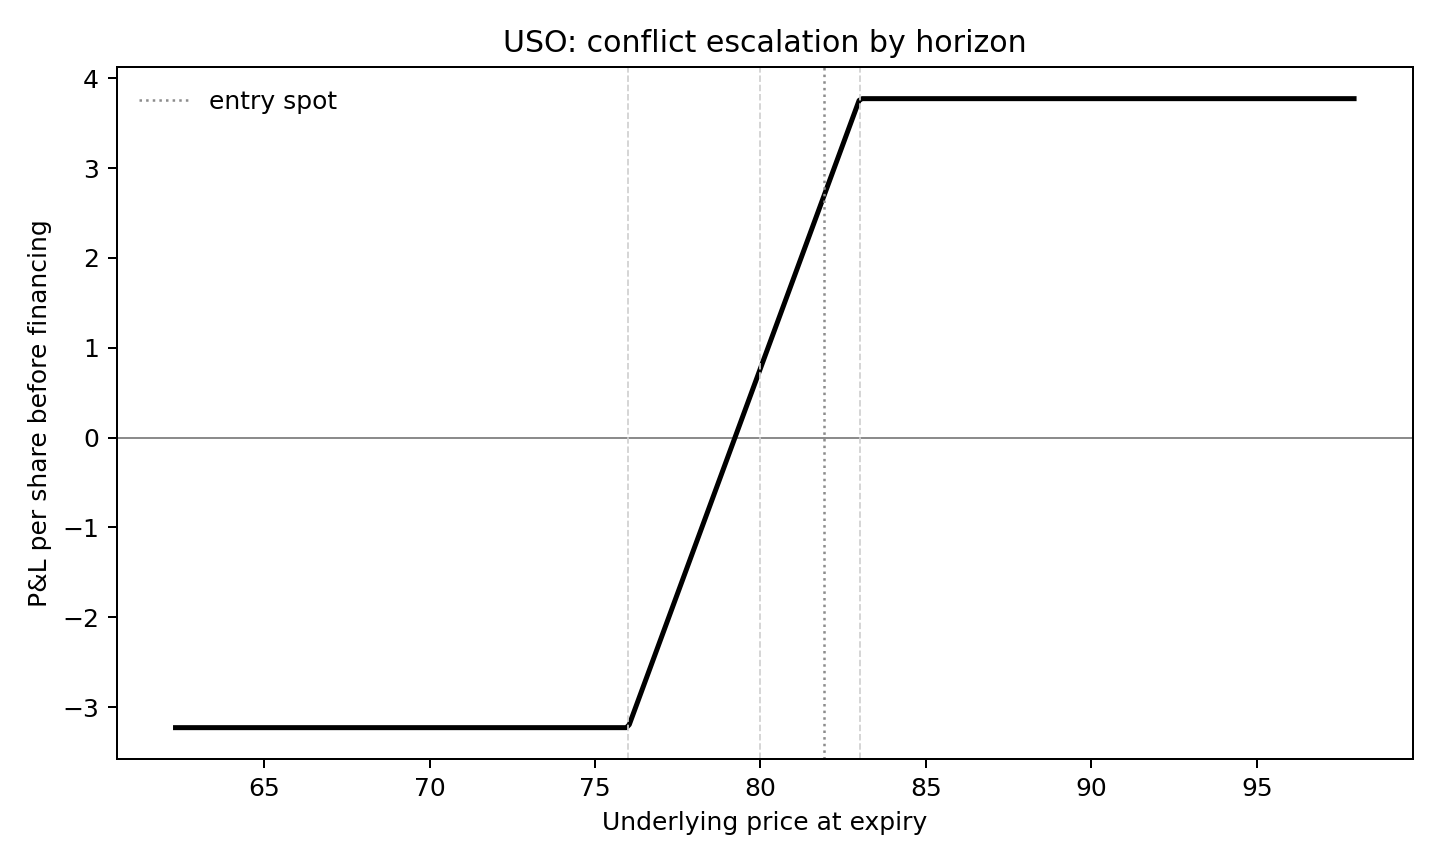
\includegraphics[width=0.86\linewidth]
    {assets/volt-event-conflict-payoff.png}
  \caption{Expiration P\&L of the pure-escalation conflict portfolio.  Two
  bounded vertical components form the payoff between strikes \(76\) and
  \(83\).}
  \label{fig:conflict-payoff}
\end{figure}

Conditional mean P\&L is \(2.7950\) under escalation and \(-0.2526\) under
the baseline.  Utility is \(2.6511\), maximum loss is \(3.2280\), and the
position's risk-adjusted break-even escalation probability is \(34\%\).
Other portfolios lead between \(34\%\) and \(41\%\); the four-leg position
becomes the global choice at \(42\%\).  Cash leads through \(17\%\).

\begin{figure}[H]
  \centering
  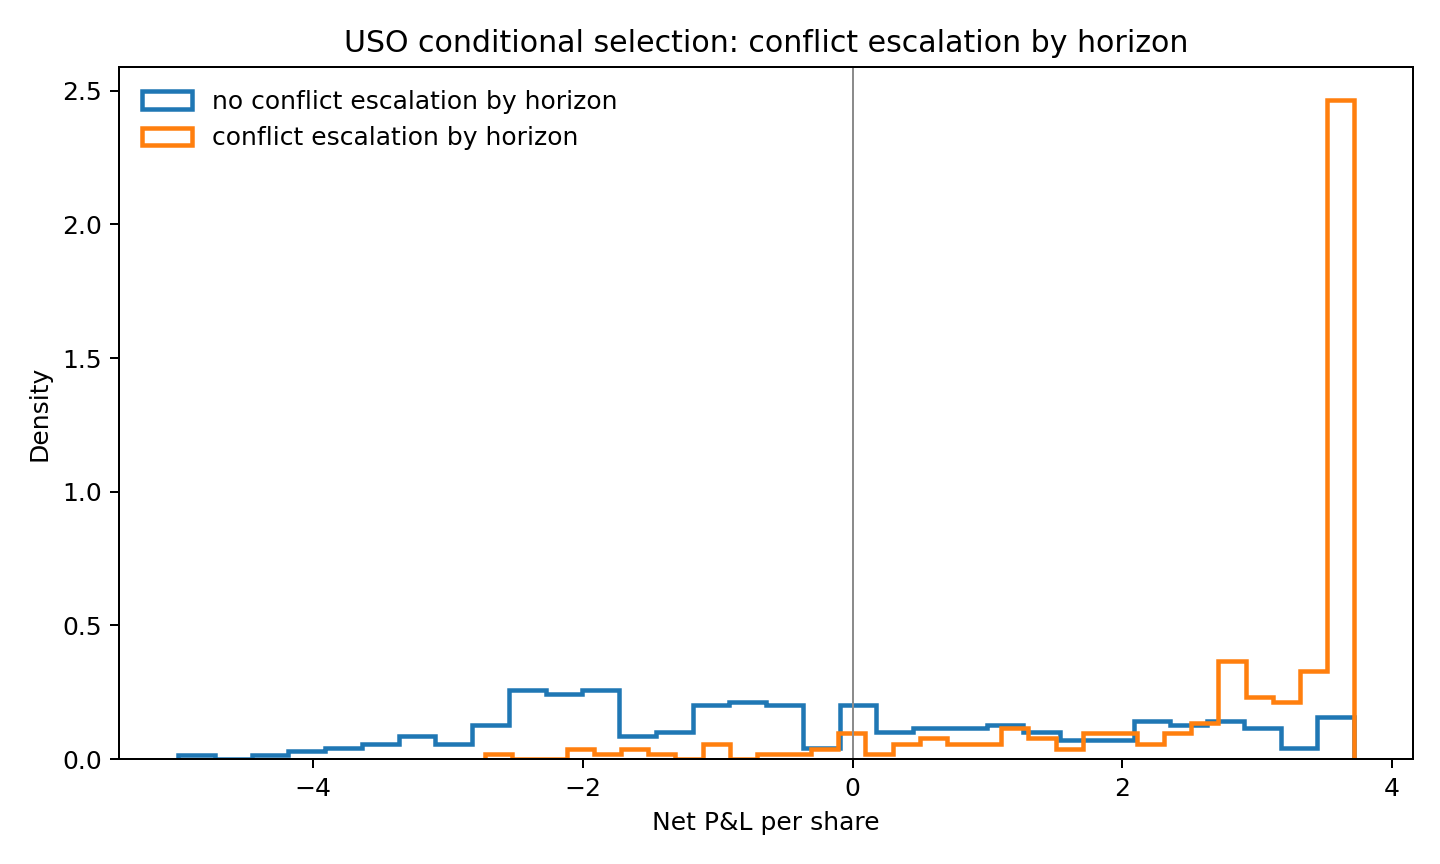
\includegraphics[width=0.87\linewidth]
    {assets/volt-event-conflict-pnl.png}
  \caption{Fixed-horizon P\&L of the four-leg conflict portfolio under the
  opposing forecast outcomes.}
  \label{fig:conflict-pnl}
\end{figure}

The four-leg position earns \(3.3640\) per share on the recorded path and is
the hindsight leader.  Forecast utility and recorded P\&L have Spearman
correlation \(0.9375\) across the retained universe.  The stated \(35\%\)
policy chooses the cheaper call spread; the larger four-leg position enters
the menu only as escalation confidence rises.

\begin{figure}[H]
  \centering
  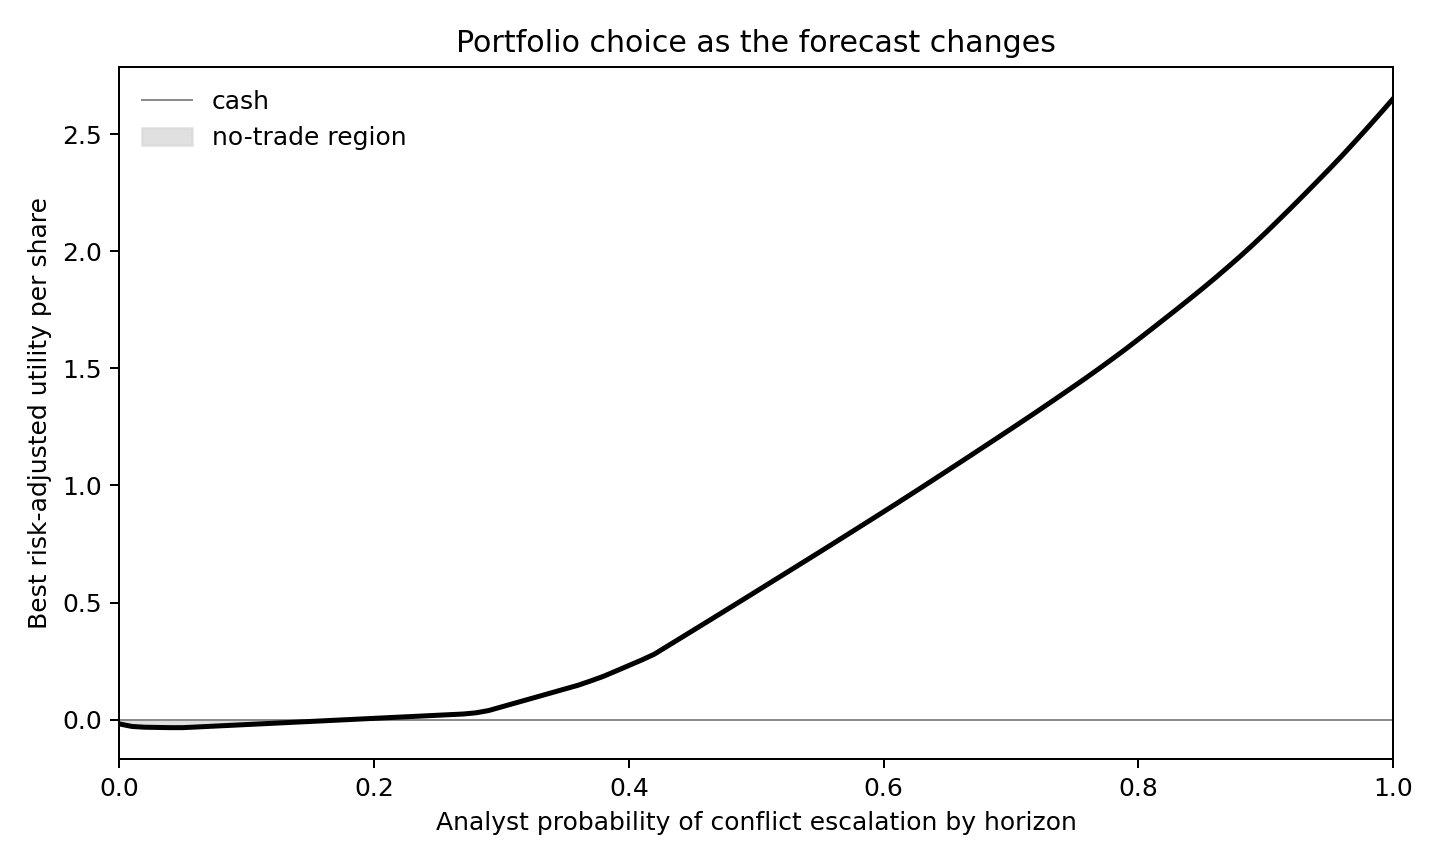
\includegraphics[width=0.88\linewidth]
    {assets/volt-event-conflict-probability.png}
  \caption{Best directional utility as conflict-escalation probability
  changes.  Cash is the policy at low probabilities.}
  \label{fig:conflict-probability}
\end{figure}

\subsection{Volatility without a directional view}

USO enters at \(61.83\%\) median IV.  Subsequent close-to-close realized
volatility is \(75.48\%\).  A \(75\%\) target is above entry IV and
therefore treats the option surface as cheap relative to the forecast.  The
selected delta-hedged position is
\[
  +C(80)-C(83)+P(78).
\]
Entry delta is \(-0.1841\), gamma \(0.08543\), daily theta \(-0.08525\),
and vega \(0.06673\).  Forecast utility is \(0.6812\), and recorded net
P\&L is \(0.9082\) per share.  Recorded gamma P\&L is \(6.4041\), theta is
\(-1.2409\), vega is \(1.4849\), and the delta hedge contributes \(2.1560\)
before the other reconciling components.

The low-volatility comparison is economically different.  At a target of
\(34.01\%\), or \(55\%\) of entry IV, the options are rich relative to the
forecast.  The preferred structure is
\(+C(80)-C(82)+P(76)-P(80)\), with entry gamma \(-0.2529\).
It has forecast utility \(0.3615\), but loses \(1.5263\) on the recorded path
as realized volatility reaches \(75.48\%\).  Its observed gamma attribution
is \(-9.5248\), partly offset by \(0.7749\) of theta.  This is the practical
meaning of conditional valuation: the short-gamma trade is attractive under
the low-vol forecast and poor under the volatility that followed.

The unrestricted optimum is short gamma at the \(61.83\%\) entry-IV grid
point and long gamma at \(71.11\%\).  The \(75\%\) forecast and subsequent
\(75.48\%\) realized volatility sit on the long-gamma side of that switch.

\begin{figure}[H]
  \centering
  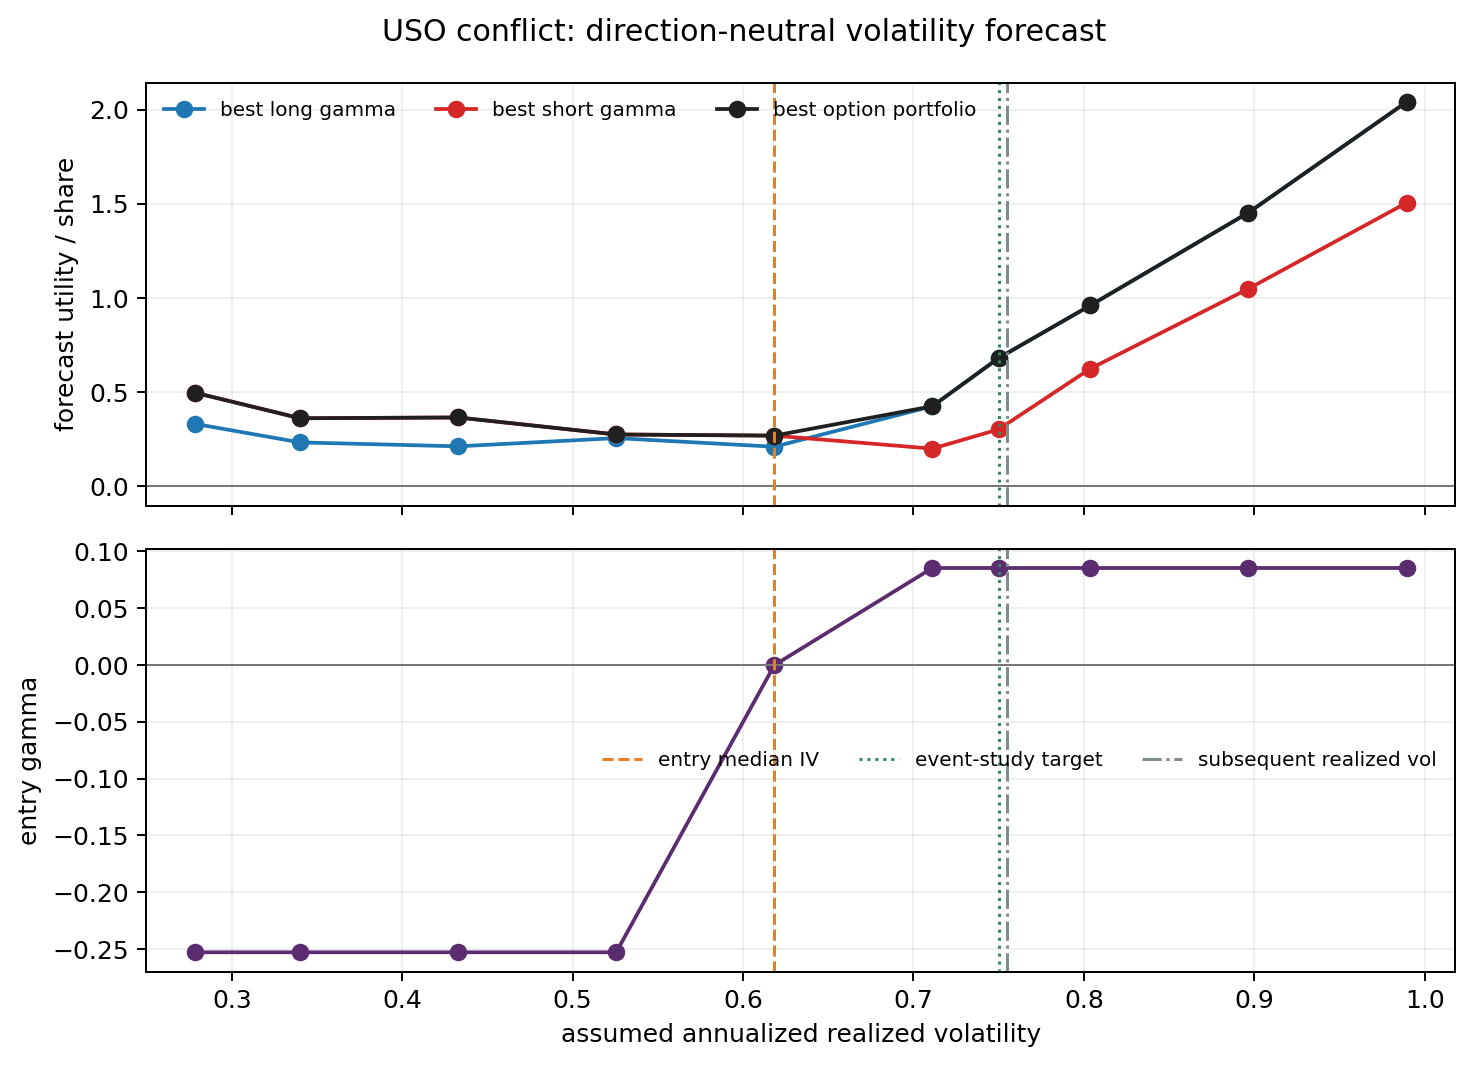
\includegraphics[width=0.90\linewidth]
    {assets/volt-event-conflict-volatility-scan.png}
  \caption{USO target-volatility scan.  The preferred exposure changes as
  the assumed realized volatility moves through the entry IV.}
  \label{fig:conflict-volatility}
\end{figure}

\section{Surrogate tests}

\subsection{Candidates held out within one date}

\begin{table}[H]
\centering
\small
\begin{tabular}{@{}llrrrr@{}}
\toprule
Study & Model & Parameters & Spearman & Top-20 & Fit seconds \\
\midrule
Tariff & Deep Sets & \(8{,}596\) & \(0.9898\) & \(20/20\) & \(0.836\) \\
Tariff & Relation GNN & \(7{,}644\) & \(0.9843\) & \(20/20\) & \(13.929\) \\
Tariff & Ridge sums & \(112\) & \(0.9685\) & \(20/20\) & \(0.003\) \\
\addlinespace
Conflict & Deep Sets & \(8{,}596\) & \(0.9715\) & \(20/20\) & \(0.417\) \\
Conflict & Relation GNN & \(7{,}644\) & \(0.9213\) & \(15/20\) & \(1.025\) \\
Conflict & Ridge sums & \(112\) & \(0.8232\) & \(14/20\) & \(0.003\) \\
\bottomrule
\end{tabular}
\caption{Single-seed candidate holdout under a common \(30\%\) label budget:
\(20\%\) initially evaluated and \(10\%\) acquired by predicted rank.}
\label{tab:models}
\end{table}

All three models recover the tariff optimum after acquisition.  The conflict
optimum happens to be present in the initial \(20\%\), so zero regret there
does not test acquisition.  These splits show interpolation among portfolios
that share one chain, spot, horizon, and scenario definition.

\subsection{A later decision date}

The chronological test changes the market state.  For tariffs, 1 April trains
the models, 7 April selects the checkpoint, and 8 April is the final
evaluation.  For conflict, the corresponding dates are 27 February, 10 March,
and 12 March.  Each date selects its liquid contracts and recompiles its
candidate universe.

\begin{table}[H]
\centering
\small
\begin{tabular}{@{}llrrrrr@{}}
\toprule
Study & Model & Spearman & Top-20 & Exact best & Mean regret & Fit sec. \\
\midrule
Tariff & Deep Sets & \(0.5166\) & \(0.0000\) & \(0/3\) & \(5.7735\) & \(1.154\) \\
Tariff & Relation GNN & \(0.7486\) & \(0.1000\) & \(0/3\) & \(0.5222\) & \(31.586\) \\
Tariff & Ridge sums & \(-0.0874\) & \(0.0333\) & \(0/3\) & \(5.2779\) & \(0.002\) \\
\addlinespace
Conflict & Deep Sets & \(-0.1053\) & \(0.0167\) & \(0/3\) & \(0.3304\) & \(0.350\) \\
Conflict & Relation GNN & \(0.5476\) & \(0.1667\) & \(0/3\) & \(0.3240\) & \(14.013\) \\
Conflict & Ridge sums & \(0.4554\) & \(0.1167\) & \(0/3\) & \(0.3084\) & \(0.001\) \\
\bottomrule
\end{tabular}
\caption{Final-date development results averaged over three event
probabilities.  Regret is the utility difference from the best evaluated
option portfolio.}
\label{tab:chronological}
\end{table}

The relation GNN gives the strongest tariff ordering and reduces mean regret
substantially relative to Deep Sets.  No model recovers a held-out optimum in
either event.  The table is also a development result: an earlier execution
exposed an input-scaling defect, and the correction was made after inspecting
that behavior.  A new, untouched date is needed for a prospective test.

\subsection{Computation}

American marks, exercise checks, and pathwise option sensitivities are
computed once per contract.  A portfolio then becomes a signed aggregation
of the compiled leg paths, followed by its hedge and account calculation.
This changes the compute comparison.

The benchmark contains 14 American options, \(12{,}313\) raw bounded
combinations, \(7{,}208\) portfolios after account filters, 64 paths, and nine
observations.  Chain construction, scenario marks, and contract-leg
compilation take \(33.317\) seconds and are shared by every method.

\begin{table}[H]
\centering
\small
\begin{tabular}{@{}rrr@{}}
\toprule
Candidates & Fixed-horizon aggregation & Daily-hedge aggregation \\
\midrule
\(250\) & \(0.221\) s & \(0.019\) s \\
\(1{,}000\) & \(0.231\) s & \(0.046\) s \\
\(4{,}000\) & \(0.225\) s & \(0.152\) s \\
\bottomrule
\end{tabular}
\caption{Portfolio computation after the common contract work.}
\label{tab:crossover-scaling}
\end{table}

At \(4{,}000\) portfolios, direct daily-hedge aggregation takes \(0.152\)
seconds.  Deep Sets search with the \(30\%\) label budget takes \(1.145\)
seconds after the shared phases; the relation GNN takes \(13.763\) seconds,
including graph export, encoding, fitting, and scoring.  End-to-end times are
\(33.470\), \(34.462\), and \(47.081\) seconds.  Deep Sets and the GNN obtain
rank correlations of \(0.9945\) and \(0.9920\), respectively.

\begin{figure}[H]
  \centering
  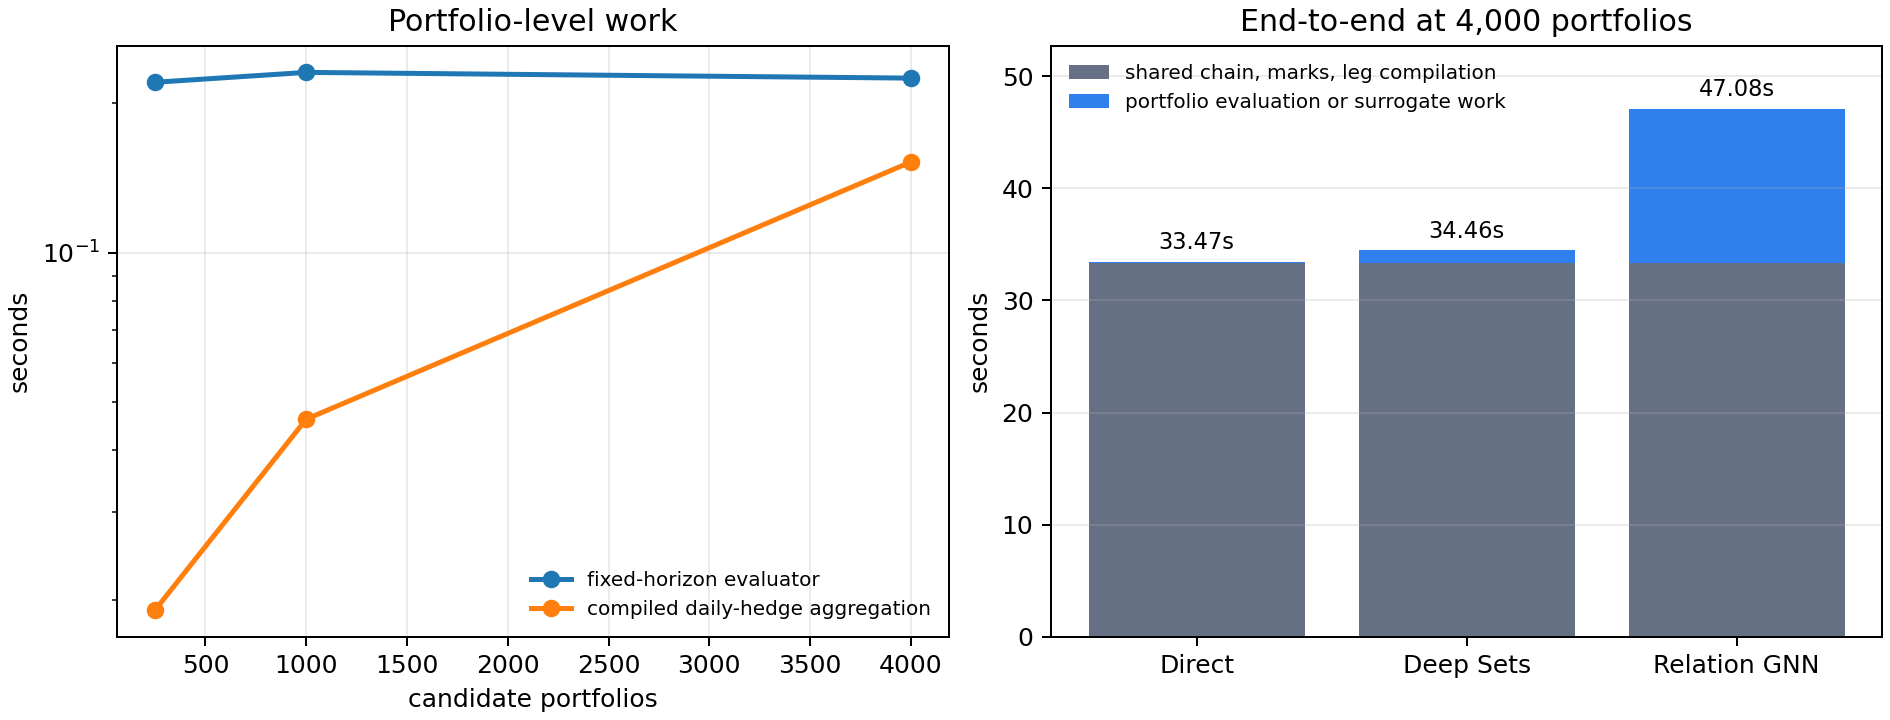
\includegraphics[width=0.74\linewidth]
    {assets/volt-compute-crossover.png}
  \caption{Compiler-aware runtime.  Direct aggregation remains faster at
  \(4{,}000\) portfolios.}
  \label{fig:compute-crossover}
\end{figure}

\section{Conclusions}

\begin{SNcolumns}

The empirical procedure begins with a point-in-time American option chain and
ends with listed quantities, entry Greeks, bounded payoff, scenario P\&L,
lifecycle events, and a cash comparison.  The directional studies show how a
probability changes both the decision to trade and the preferred structure.
The volatility studies answer a separate question: with median return fixed
at zero, a target below entry IV favors bounded short gamma, while a target
above entry IV favors long convexity after daily hedging and costs.

The learning results are more limited.  Within one date, both neural
representations fit the portfolio ranking well.  Across dates, the ordering
weakens and the best candidate is missed.  Compiled direct evaluation is
faster for the candidate counts measured here.  More independent decision
dates are therefore required before a learned shortlist can replace direct
evaluation.

A later sequential study can admit conditional close, roll, exercise, hedge,
inventory, and account actions.  Those actions change later holdings, legal
actions, and transaction costs; they are the setting in which a graph state
and reinforcement learning may add value.  That proposition requires its
own empirical test.

\end{SNcolumns}

\begin{thebibliography}{9}

\bibitem{crr}
J. C. Cox, S. A. Ross, and M. Rubinstein.
\newblock Option pricing: a simplified approach.
\newblock \emph{Journal of Financial Economics}, 7(3):229--263, 1979.

\bibitem{deepsets}
M. Zaheer, S. Kottur, S. Ravanbakhsh, B. P\'oczos, R. Salakhutdinov,
and A. Smola.
\newblock Deep Sets.
\newblock \emph{Advances in Neural Information Processing Systems}, 2017.
\newblock \url{https://arxiv.org/abs/1703.06114}.

\bibitem{graphnetworks}
P. W. Battaglia et al.
\newblock Relational inductive biases, deep learning, and graph networks.
\newblock arXiv:1806.01261, 2018.
\newblock \url{https://arxiv.org/abs/1806.01261}.

\bibitem{crs-tariffs}
Congressional Research Service.
\newblock Presidential 2025 tariff actions: timeline and status.
\newblock Report R48549, updated 2026.
\newblock \url{https://www.congress.gov/crs-product/R48549}.

\bibitem{strategynet-tariffs}
StrategyNet.
\newblock ``Liberation Day'' tariffs: market response to the announcement
and court ruling.
\newblock 12 July 2026.
\newblock
\url{https://strategynet.ai/insights/liberation-day-tariffs-factor-evolution}.

\bibitem{strategynet-conflict}
StrategyNet.
\newblock US--Israel/Iran conflict (Feb.\ 28--Mar.\ 9, 2026): from factor
shock to a risk-adjusted portfolio.
\newblock 12 July 2026.
\newblock
\url{https://strategynet.ai/insights/us-iran-conflict-factor-evolution-2026}.

\bibitem{ap-conflict}
Associated Press.
\newblock A timeline of the Iran conflict and talks aimed at ending it.
\newblock July 2026.
\newblock
\url{https://apnews.com/article/iran-us-timeline-trump-hormuz-war-ceasefire-04da58cbae991183f8b52ef5bf615963}.

\bibitem{occ}
Options Clearing Corporation.
\newblock Options strategies quick guide.
\newblock
\url{https://www.theocc.com/getcontentasset/f34f8a0d-806f-4f1a-adf7-d49d8d94b16e/dfc3d011-8f63-43f6-9ed8-4b444333a1d0/option-strategies-quick-guide.pdf}.

\end{thebibliography}

\end{document}
